\documentclass{article}

\usepackage[utf8]{inputenc}
\usepackage[bottom=2cm, top=2cm, left=2cm, right=2cm]{geometry}
\usepackage{verbatim}
\usepackage{tikz}

\title{Lista - Árvores B}
\author{Vinícius Couto Tasso}
\date{}

\begin{document}

\maketitle
\tikzset{every tree node/.style={minimum width=2em,draw,circle},
         blank/.style={draw=none},
         edge from parent/.style=
         {draw,edge from parent path={(\tikzparentnode) -- (\tikzchildnode)}},
         level distance=1cm}
         
\begin{enumerate}

\item \textbf{Por que não permitimos um grau mínimo de $t = 1$ em uma árvore B?}

Por definição, uma árvore B deve ter pelo menos $t - 1$ chaves (propriedade 5a) em todos seus nós diferentes da raiz. Com $t = 1$, seria permitido nós que não contém chave alguma e, consequentemente, nós com apenas 1 filho (o que não faz sentido para árvores binárias).

\item \textbf{Para que valores de $t$ a árvore abaixo é uma árvore B válida?}

A árvore é valida para $t = 2$ e $t = 3$.

\item \textbf{Mostre todas as árvores B válidas de grau mínimo 2 que representam \{1,2,3,4,5\}.}


\begin{center}
    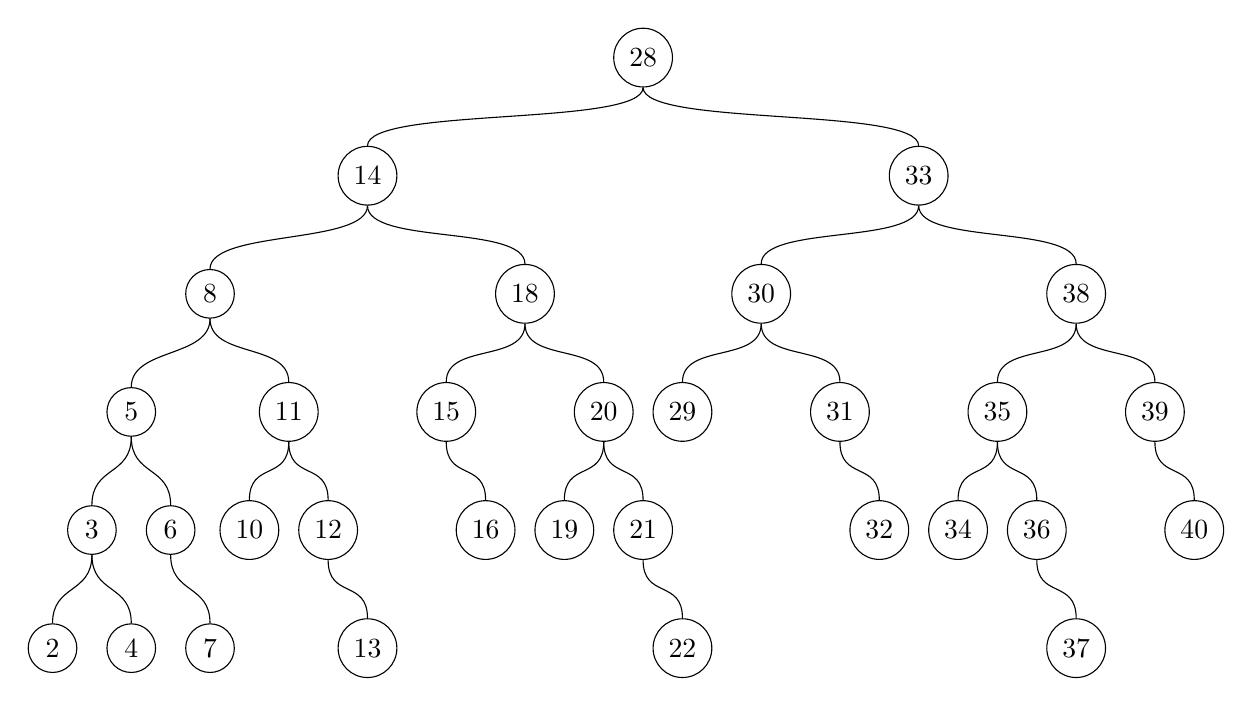
\begin{tikzpicture}[
       edge from parent path=
    {(\tikzparentnode.south) .. controls +(0,-.5) and +(0,.5)
                             .. (\tikzchildnode.north)},
    level 1/.style={sibling distance=7cm},                        
    level 2/.style={sibling distance=4cm},                         
    level 3/.style={sibling distance=2cm},
    level 4/.style={sibling distance=1cm},
   every node/.style={draw,circle},
   label distance=-1mm]
   
\node {28}
    child {node {14}
        child {node {8}
            child {node {5}
                child {node {3}
                    child {node {2}}
                    child {node {4}}
                }
                child {node {6}
                    child[missing] {}
                    child {node {7}}
                }
            }
            child {node {11}
                child {node {10}}
                child {node {12}
                    child[missing] {}   
                    child {node {13}}
                }
            }
        }
        child {node {18}
            child {node {15}
                child[missing] {}   
                child {node {16}}
            }
            child {node {20}
                child {node {19}}
                child {node {21}
                    child[missing] {}   
                    child {node {22}}
                }
            }
        }
    }   
    child {node {33}
        child {node {30}
            child {node {29}}
            child {node {31}
                    child[missing] {}
                    child {node {32}}
                }
            }
        child {node {38}
            child {node {35}
                child {node {34}}
                child {node {36}
                    child[missing] {}
                    child {node {37}}
                }
            }
            child {node {39}
                child[missing] {}
                child {node {40}}
            }
        }
    };

\end{tikzpicture}
\end{center}

\item \textbf{Mostre o resultado da inserção das chaves}

\begin{verbatim}
    F, S, Q, K, C, L, H, T, V, W, M, R, N, P, A, B, X, Y, D, Z, E
\end{verbatim}
\textbf{nessa ordem em uma árvore B vazia com grau mínimo 2. Desenhe apenas as configurações da árvore imediatamente antes de ter de dividir nó, e desenhe também a configuração final.}

\begin{center}
    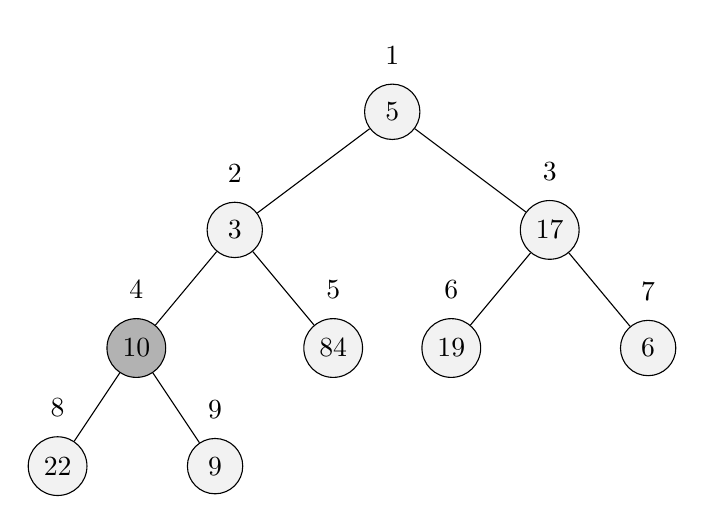
\begin{tikzpicture}
   \tikzstyle{level 1}=[sibling distance=4cm]
   \tikzstyle{level 2}=[sibling distance=2.5cm]
   \tikzstyle{level 3}=[sibling distance=2cm]
   \tikzstyle{every node}=[draw, circle, fill=gray, fill opacity=0.1, text opacity=1, minimum size=2em]
   
\node[label=90:$1$] {5}
    child {node[label=90:$2$] {3}
        child {node[label=90:$4$, fill=black, fill opacity=0.3] {10}
            child {node[label=90:$8$] {22}}
            child {node[label=90:$9$] {9}}
        }
        child {node[label=90:$5$] {84}}
    }
    child {node[label=90:$3$] {17}
        child {node[label=90:$6$] {19}}
        child {node[label=90:$7$] {6}}
    };

\end{tikzpicture}
\end{center}

\begin{center}
    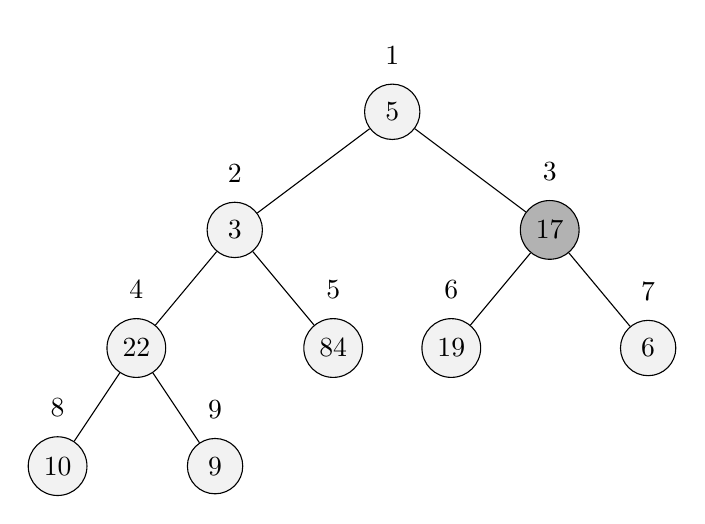
\begin{tikzpicture}
   \tikzstyle{level 1}=[sibling distance=4cm]
   \tikzstyle{level 2}=[sibling distance=2.5cm]
   \tikzstyle{level 3}=[sibling distance=2cm]
   \tikzstyle{every node}=[draw, circle, fill=gray, fill opacity=0.1, text opacity=1, minimum size=2em]
   
\node[label=90:$1$] {5}
    child {node[label=90:$2$] {3}
        child {node[label=90:$4$] {22}
            child {node[label=90:$8$] {10}}
            child {node[label=90:$9$] {9}}
        }
        child {node[label=90:$5$] {84}}
    }
    child {node[label=90:$3$, fill=black, fill opacity=0.3] {17}
        child {node[label=90:$6$] {19}}
        child {node[label=90:$7$] {6}}
    };

\end{tikzpicture}
\end{center}

\begin{center}
    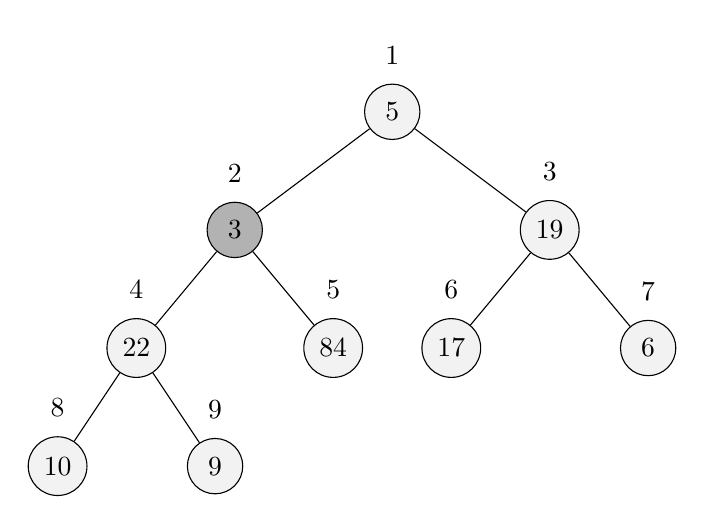
\begin{tikzpicture}
   \tikzstyle{level 1}=[sibling distance=4cm]
   \tikzstyle{level 2}=[sibling distance=2.5cm]
   \tikzstyle{level 3}=[sibling distance=2cm]
   \tikzstyle{every node}=[draw, circle, fill=gray, fill opacity=0.1, text opacity=1, minimum size=2em]
   
\node[label=90:$1$] {5}
    child {node[label=90:$2$, fill=black, fill opacity=0.3] {3}
        child {node[label=90:$4$] {22}
            child {node[label=90:$8$] {10}}
            child {node[label=90:$9$] {9}}
        }
        child {node[label=90:$5$] {84}}
    }
    child {node[label=90:$3$] {19}
        child {node[label=90:$6$] {17}}
        child {node[label=90:$7$] {6}}
    };

\end{tikzpicture}
\end{center}

\begin{center}
    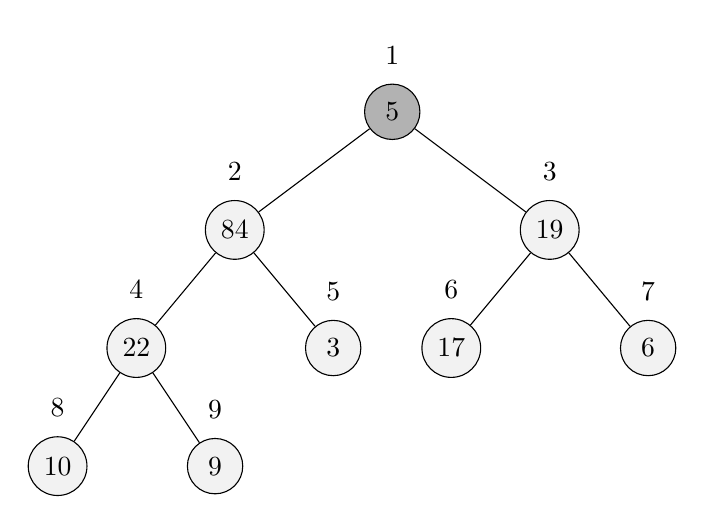
\begin{tikzpicture}
   \tikzstyle{level 1}=[sibling distance=4cm]
   \tikzstyle{level 2}=[sibling distance=2.5cm]
   \tikzstyle{level 3}=[sibling distance=2cm]
   \tikzstyle{every node}=[draw, circle, fill=gray, fill opacity=0.1, text opacity=1, minimum size=2em]
   
\node[label=90:$1$, fill=black, fill opacity=0.3] {5}
    child {node[label=90:$2$] {84}
        child {node[label=90:$4$] {22}
            child {node[label=90:$8$] {10}}
            child {node[label=90:$9$] {9}}
        }
        child {node[label=90:$5$] {3}}
    }
    child {node[label=90:$3$] {19}
        child {node[label=90:$6$] {17}}
        child {node[label=90:$7$] {6}}
    };

\end{tikzpicture}
\end{center}

\begin{center}
    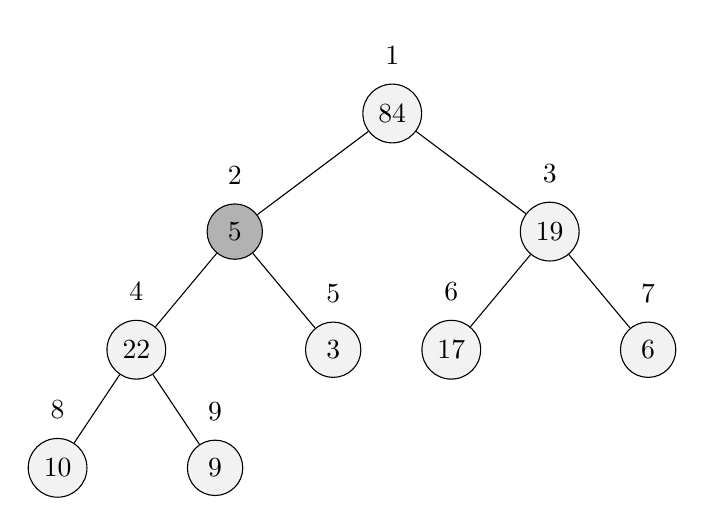
\begin{tikzpicture}
   \tikzstyle{level 1}=[sibling distance=4cm]
   \tikzstyle{level 2}=[sibling distance=2.5cm]
   \tikzstyle{level 3}=[sibling distance=2cm]
   \tikzstyle{every node}=[draw, circle, fill=gray, fill opacity=0.1, text opacity=1, minimum size=2em]
   
\node[label=90:$1$] {84}
    child {node[label=90:$2$, fill=black, fill opacity=0.3] {5}
        child {node[label=90:$4$] {22}
            child {node[label=90:$8$] {10}}
            child {node[label=90:$9$] {9}}
        }
        child {node[label=90:$5$] {3}}
    }
    child {node[label=90:$3$] {19}
        child {node[label=90:$6$] {17}}
        child {node[label=90:$7$] {6}}
    };

\end{tikzpicture}
\end{center}

\begin{center}
    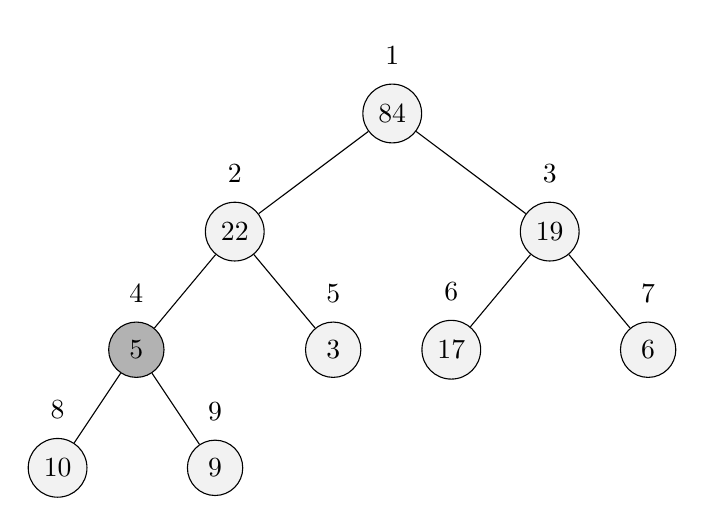
\begin{tikzpicture}
   \tikzstyle{level 1}=[sibling distance=4cm]
   \tikzstyle{level 2}=[sibling distance=2.5cm]
   \tikzstyle{level 3}=[sibling distance=2cm]
   \tikzstyle{every node}=[draw, circle, fill=gray, fill opacity=0.1, text opacity=1, minimum size=2em]
   
\node[label=90:$1$] {84}
    child {node[label=90:$2$] {22}
        child {node[label=90:$4$, fill=black, fill opacity=0.3] {5}
            child {node[label=90:$8$] {10}}
            child {node[label=90:$9$] {9}}
        }
        child {node[label=90:$5$] {3}}
    }
    child {node[label=90:$3$] {19}
        child {node[label=90:$6$] {17}}
        child {node[label=90:$7$] {6}}
    };

\end{tikzpicture}
\end{center}

\begin{center}
    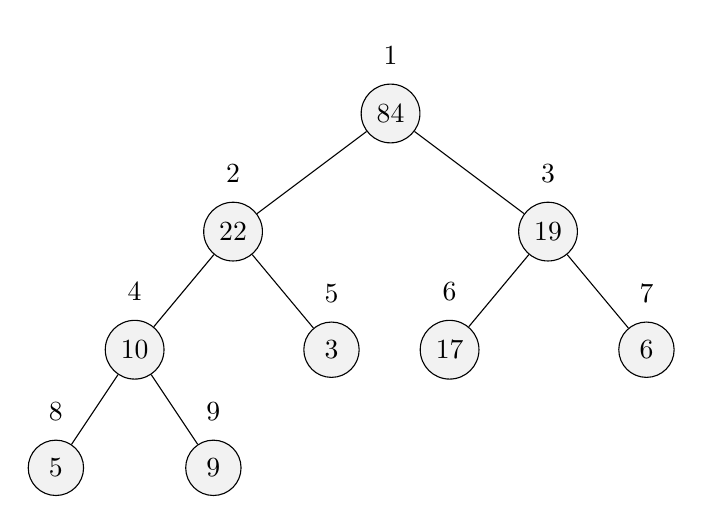
\begin{tikzpicture}
   \tikzstyle{level 1}=[sibling distance=4cm]
   \tikzstyle{level 2}=[sibling distance=2.5cm]
   \tikzstyle{level 3}=[sibling distance=2cm]
   \tikzstyle{every node}=[draw, circle, fill=gray, fill opacity=0.1, text opacity=1, minimum size=2em]
   
\node[label=90:$1$] {84}
    child {node[label=90:$2$] {22}
        child {node[label=90:$4$] {10}
            child {node[label=90:$8$] {5}}
            child {node[label=90:$9$] {9}}
        }
        child {node[label=90:$5$] {3}}
    }
    child {node[label=90:$3$] {19}
        child {node[label=90:$6$] {17}}
        child {node[label=90:$7$] {6}}
    };

\end{tikzpicture}
\end{center}

\end{enumerate}

\end{document}
